\documentclass{TDP003mall}
\usepackage{titlesec}
\usepackage{graphicx}
\definecolor{terminalgreen}{HTML}{8AE234}

\newcommand{\version}{Version 0.1}
\author{Eric Jönsson, \url{erijo137@student.liu.se}\\
  Ida Bergquist, \url{idabe112@student.liu.se}}
\title{Systemdocumentation}
\date{2018-10-16}
\rhead{Ida Bergquist\\
Eric Jönsson}



\begin{document}
\projectpage
\tableofcontents
\newpage
\section{Revisions}
\begin{table}[!h]
\begin{tabularx}{\linewidth}{|l|X|l|}
\hline
\textbf{Ver.} & \textbf{Description of revisions} & \textbf{Datum} \\\hline
0.1 & First version created & 181016 \\\hline
\end{tabularx}
\end{table}

\section{Overview}
\begin{figure}[h!]
    \centering
    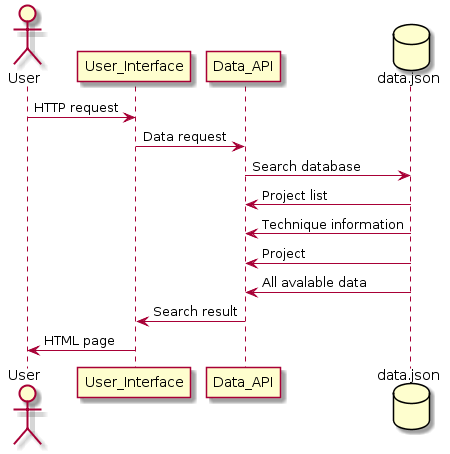
\includegraphics[width=10cm]{sevenskdiagram.png}
    \caption{Simplified view of the portfolio}
    \label{sekvensdiagram}
\end{figure}
In broad terms, the portfolio functions by the user interface taking request from the user and then sends a query to the data API for data needed to create the reqested html-page.
The user interface sends specific requests to the data API depending on what data is needed to build the html-page.
\section{Design}
\subsection{Data API}
All functions are defined in a seperate document called module documentation.
\newpage
\subsection{User interface}
\begin{figure}[h!]
    \centering
    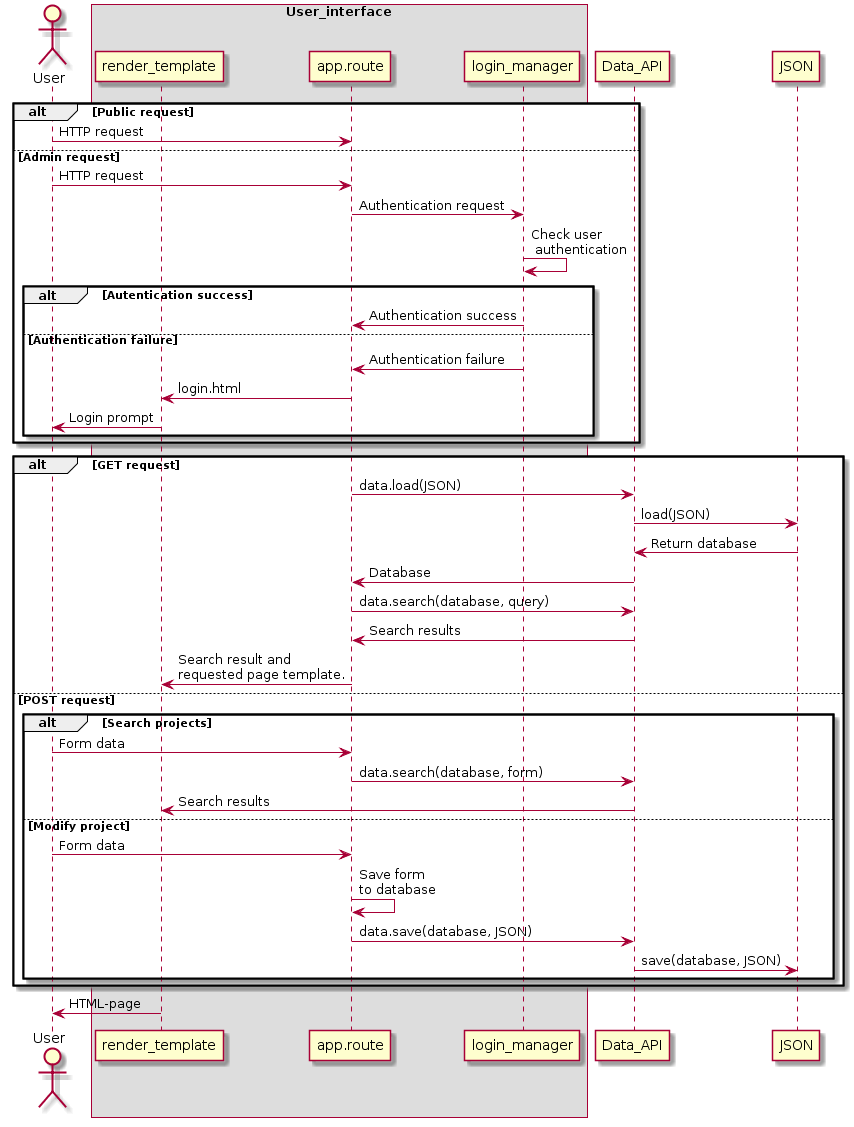
\includegraphics[width=14cm]{sekvensdiagram2-3.png}
    \caption{The inner workings of the user interface}
    \label{sekvensdiagram2}
\end{figure}
All functions are defined in a seperate document called module documentation.

\newpage
\section{Errors and errorlogs}


\end{document}
